\chapter{\texorpdfstring{相干函数 $g^{(1)}$、$g^{(2)}$ 与 Siegert 关系}{相干函数 g1、g2 与 Siegert 关系}}
\label{chap:e08}

\begin{chapteropening}
到这里，望远镜交给我们的已经不再是"一团亮度"，而是第 \ref{chap:e07} 章讲的那张\textbf{事件表}（event list）：一串带时间戳的"点击"。现在要问的，不再是"平均有多亮"，而是一个更微妙的问题——\emph{这些点击彼此之间，有没有关系？}如果两个探测器、两个时间门里的光子只是各自随机地到来，那么它们偶尔一起响一下，纯属巧合；可如果它们\emph{比巧合更常}一起响，或者\emph{比巧合更少}一起响，事件表里就藏着光场统计的指纹。本章要教你一套把"事件表"翻译成"光场统计"的语言：一阶相干 \(g^{(1)}\) 量的是电场的相位记忆，二阶相干 \(g^{(2)}\) 量的是光子结伴到达的倾向。而把这两者接通的，是本章的高潮——Siegert 关系。它会告诉你一件近乎魔法的事：只靠数强度涨落的"同步程度"，就能读出电场相干度的模平方。这正是后面强度干涉与成像的全部底气。
\end{chapteropening}

\section{为什么要给"相关"一个函数}
\label{sec:e08-why-correlation}

先把上一阶段的结论接住。第 \ref{chap:e02} 章告诉我们：光只在一个很短的相干时间 \(\tau_c\) 内"记得"自己的相位，可见光宽带下 \(\tau_c\) 短到皮秒；探测器却慢到百皮秒以上，一个时间门里平均了成百上千段互不相干的波列。第 \ref{chap:e06} 章又告诉我们，不同的光态（相干态、热态、数态）即便平均亮度一模一样，光子数的\emph{起伏}却天差地别。把这两条放在一起，一个自然的念头就冒出来了：\emph{既然一次曝光的总强度抹掉了这么多信息，我们能不能不看"总量"，改看"两次探测之间的呼应"？}

这正是相干函数（coherence function）的用武之地。它的思路极其朴素，和第 \ref{chap:e02} 章的自相关函数一脉相承：把光场（或光子流）和"延迟了 \(\tau\) 的自己"放在一起比较，看它们还有多像。区别只在于"比较什么"：

\begin{itemize}
  \item 若比较的是\textbf{电场振幅与相位}，得到的是一阶相干 \(g^{(1)}(\tau)\)——它回答"电场隔了 \(\tau\) 还记得多少相位"。振幅干涉（第 \ref{chap:e09} 章）用的就是它。
  \item 若比较的是\textbf{强度（光子到达）}，得到的是二阶相干 \(g^{(2)}(\tau)\)——它回答"两个探测事件是不是比随机情形更爱成对出现"。Hanbury Brown--Twiss（HBT）强度干涉用的就是它 \citep{1956Natur.177...27B}。
\end{itemize}

之所以要把"相关"写成一个\emph{关于延迟 \(\tau\) 的函数}，而不是一个数，是因为呼应的强弱随延迟变化：延迟很小时呼应最强，延迟拉长到超过相干时间，两次探测就彻底"失联"了。这条呼应随 \(\tau\) 衰减的曲线，它的\emph{高度}和\emph{宽度}里，分别编码着光的种类（热光还是激光）和光的谱宽（相干时间）。本章就是要把这两条曲线一根一根讲清楚，再把它们用一座桥——Siegert 关系——连起来。

\section{一阶相干：电场隔着 \texorpdfstring{$\tau$}{tau} 还记得多少相位}
\label{sec:e08-g1}

先看最容易想象的一阶。第 \ref{chap:e05} 章我们把探测面上的正频率电场写成算符 \(\hat E^{(+)}(t)\)（它只含湮灭算符 \(\hat a\)，作用是"减少一个光子"），它的厄米共轭 \(\hat E^{(-)}(t)\)（只含产生算符 \(\hat a^\dagger\)）是负频率部分。一阶相干函数定义为把两个时刻的场"相乘再平均"：

\begin{equation}
  G^{(1)}(t_1,t_2)=\big\langle \hat E^{(-)}(t_1)\,\hat E^{(+)}(t_2)\big\rangle,
  \qquad
  g^{(1)}(\tau)=\frac{G^{(1)}(t,t+\tau)}{G^{(1)}(t,t)} .
  \label{eq:e08-g1}
\end{equation}
\begin{formulaexplain}
\(G^{(1)}\) 是一阶场相关；\(\hat E^{(+)},\hat E^{(-)}\) 是正、负频率场算符；\(\langle\cdot\rangle\) 是量子态上的期望；\(g^{(1)}\) 是把它除以零延迟值后的归一化版本；\(\tau=t_2-t_1\) 是延迟。它测电场隔 \(\tau\) 还留多少相位记忆。
\end{formulaexplain}

逐个符号落实。\(G^{(1)}(t,t)=\langle\hat E^{(-)}(t)\hat E^{(+)}(t)\rangle\) 就是 \(t\) 时刻的平均强度（正实数，带强度量纲），所以归一化后的 \(g^{(1)}\) 是无量纲的复数。若光场是\emph{平稳的}（statistically stationary，统计性质不随绝对时间漂移，这是稳定光源的常态），相关只依赖延迟 \(\tau\)，与起点 \(t\) 无关，于是 \(g^{(1)}\) 只是 \(\tau\) 的函数。它的模 \(|g^{(1)}(\tau)|\) 落在 \([0,1]\) 之间，物理含义一句话就能抓住：

\begin{itemize}
  \item \(|g^{(1)}(\tau)|\to1\)：延迟 \(\tau\) 之后的电场，仍和原来的电场步调一致、相位可预测——\textbf{相干}。把它和延迟前的自己叠加，会拉出清晰的干涉条纹。
  \item \(|g^{(1)}(\tau)|\to0\)：电场已经把 \(\tau\) 之前的相位忘得干干净净——\textbf{失忆}。此时叠加得到的是一片糊掉的、没有条纹的亮度。
\end{itemize}

这正是第 \ref{chap:e02} 章自相关函数 \(\Gamma(\tau)\) 的"电场版"：\(g^{(1)}(\tau)\) 从峰值 1 衰减到 0 的宽度，就是相干时间 \(\tau_c\)。而 \(\tau_c\) 由谱宽定，回忆第 \ref{chap:e02} 章的两条式子：

\begin{equation}
  \Delta\nu\simeq\frac{c\,\Delta\lambda}{\lambda^2},
  \qquad
  \tau_c\simeq\frac{1}{\Delta\nu}\simeq\frac{\lambda^2}{c\,\Delta\lambda}.
  \label{eq:e08-tauc}
\end{equation}
\begin{formulaexplain}
\(\Delta\nu\) 是频率带宽（Hz），\(\Delta\lambda\) 是波长带宽，\(\lambda\) 是中心波长，\(c\) 是光速，\(\tau_c\) 是相干时间（s）。它把"滤光片有多窄"直接换算成"电场相位记忆有多久"。
\end{formulaexplain}

代进真实数字体会一下量级。取一片"很窄"的滤光片：中心波长 \(\lambda=780\,{\rm nm}\)、带宽 \(\Delta\lambda=1\,{\rm nm}\)。先算频率带宽（用 CGS，\(c=3\times10^{10}\,{\rm cm\,s^{-1}}\)，\(\lambda=7.8\times10^{-5}\,{\rm cm}\)，\(\Delta\lambda=10^{-7}\,{\rm cm}\)）：
\[
  \Delta\nu\simeq\frac{(3\times10^{10})(10^{-7})}{(7.8\times10^{-5})^2}
  =\frac{3\times10^{3}}{6.1\times10^{-9}}
  \approx4.9\times10^{11}\,{\rm Hz},
\]
于是
\[
  \tau_c\simeq\frac{1}{4.9\times10^{11}\,{\rm Hz}}\approx2\times10^{-12}\,{\rm s}=2\,{\rm ps}.
\]
也就是说，即便隔着一片 1 纳米的窄带滤光片，恒星热光的电场也只记得自己约 2 皮秒的相位，然后就翻篇了。这个 2 ps 会在本章反复出现，并直接决定后面强度相关峰有多窄、被稀释多少倍。

\section{二阶相干：光子是否喜欢结伴到达}
\label{sec:e08-g2}

把问题从"电场是否还记得相位"换成"两个探测事件是否相关"，就进入二阶。量子光电探测理论（第 \ref{chap:e07} 章）给出的定义，是四个场算符按一种特定次序排好后取平均：

\begin{equation}
  G^{(2)}(t_1,t_2)=\big\langle
    \hat E^{(-)}(t_1)\,\hat E^{(-)}(t_2)\,\hat E^{(+)}(t_2)\,\hat E^{(+)}(t_1)
  \big\rangle,
  \qquad
  g^{(2)}(\tau)=\frac{G^{(2)}(t,t+\tau)}{G^{(1)}(t,t)\,G^{(1)}(t+\tau,t+\tau)} .
  \label{eq:e08-g2-field}
\end{equation}
\begin{formulaexplain}
\(G^{(2)}\) 是二阶场相关；四个算符里两个产生（\(\hat E^{(-)}\)）全排在左边、两个湮灭（\(\hat E^{(+)}\)）全排在右边，这叫\textbf{正规序}（normal order）；至于内外那层嵌套，是按时间配对的（\(t_1\) 一对在最外层、\(t_2\) 一对在里层），保证"先在 \(t_1\) 吸收、再在 \(t_2\) 吸收"的时间序。分母是两个时刻各自的平均强度之积；\(g^{(2)}\) 是归一化结果。它测光子是否倾向成对到达。
\end{formulaexplain}

这条式子值得逐项慢慢读，因为每一项都对应事件表里一个能数出来的东西。

\textbf{为什么是这个奇怪的算符次序？}第 \ref{chap:e07} 章讲过，探测器"数"的是\emph{吸收}一个光子的事件，每吸收一个就用掉一个湮灭算符 \(\hat E^{(+)}\)。要在 \(t_1\) 和 \(t_2\) 两个时刻各探到一个光子，就要连用两个湮灭算符 \(\hat E^{(+)}(t_2)\hat E^{(+)}(t_1)\) 作用在态上，得到态矢 \(\hat E^{(+)}(t_2)\hat E^{(+)}(t_1)|\psi\rangle\)；这个联合探测的概率正是它的模平方 \(\big|\hat E^{(+)}(t_2)\hat E^{(+)}(t_1)|\psi\rangle\big|^2\)，展开来就是把两个产生算符原样搬到左边。于是产生算符全排在左边、湮灭算符全排在右边——这就是正规序，它保证我们数的是\emph{两个不同的吸收事件}，而不是同一个光子和自己配对的假项。至于公式里"外/内"那层嵌套，纯粹来自时间配对：带 \(t_1\) 的一对（一个产生、一个湮灭）在最外层，带 \(t_2\) 的一对在里层，锁定"先在 \(t_1\) 吸收、再在 \(t_2\) 吸收"的时间顺序，与"产生在左、湮灭在右"是两件不同的事，别把它们混为一谈。这一点在第 \ref{chap:e07} 章的阶乘矩 \(\langle N(N-1)\rangle\) 里已经埋下伏笔：探测器允许的是不同光子组成的有序对。

\textbf{分母是什么？}分母 \(G^{(1)}(t,t)\,G^{(1)}(t+\tau,t+\tau)=\langle I(t)\rangle\langle I(t+\tau)\rangle\)，是"假设两个探测完全独立时，随机符合应该有多少"的基线。换句话说，如果两个时刻的光子毫不相干，各自按自己的平均率随机到来，那么它们碰巧一起被探到的联合率，就是两个平均率相乘。

\textbf{分子是什么？}分子是真实的\emph{共同}探测强度。把它除以那条"独立时的随机符合基线"，\(g^{(2)}\) 就成了一个无量纲的\emph{相对过量}：

\begin{itemize}
  \item \(g^{(2)}(\tau)=1\)：真实符合恰好等于随机基线，光子的到来彼此独立。理想激光（相干态，第 \ref{chap:e06} 章）就是这样——它给出泊松（Poisson）计数，\(g^{(2)}=1\)。
  \item \(g^{(2)}(0)>1\)：零延迟附近的光子对\emph{比随机更多}，光子爱扎堆，叫\textbf{聚束}（bunching）。理想单模热光给出漂亮的 \(g^{(2)}(0)=2\)。
  \item \(g^{(2)}(0)<1\)：零延迟符合被\emph{压低}，光子彼此回避，叫\textbf{反聚束}（antibunching）。这一条无法由任何正定的经典强度涨落解释，是单光子源、共振荧光的标准\emph{非经典}判据 \citep{1977PhRvL..39..691K}。
\end{itemize}

理想单模热光为什么恰好是 2？物理图像在第 \ref{chap:e06} 章已经埋好：热光的电场是许多随机相位的小贡献叠加，瞬时强度会形成随机的明暗斑纹；探测器在"亮斑"里更容易接连记录多个光子，于是零延迟附近符合升高。而 2 这个具体数字，正是下一节 Siegert 关系在 \(\tau=0\) 处的直接推论——先记住这个悬念。

在工程估算里，人们常把同一件事写成连续强度的形式：

\begin{equation}
  g^{(2)}(\tau)=\frac{\big\langle I(t)\,I(t+\tau)\big\rangle}{\big\langle I(t)\big\rangle^2}.
  \label{eq:e08-g2-classical}
\end{equation}
\begin{formulaexplain}
\(I(t)\) 是强度（或正比于它的探测电流、计数率）；分子是两时刻强度的共同涨落；分母是平均强度的平方（用了平稳性，两个时刻的平均相同）。这是二阶相干的"经典写法"，便于估算。
\end{formulaexplain}

这行式子方便，但埋着一个必须点破的\textbf{陷阱}：\(I(t)\) 到底是哪一个强度？它可以是光场理想的\emph{瞬时}强度，也可以是探测器输出的电流、TDC 记录的事件率或采样后的 ADC 值。这两者天差地别——后者已经被探测器几纳秒的响应\emph{卷积}过了。如果你把一个被 4 ns 电子响应抹平后的 \(I(t)\) 代进式 \eqref{eq:e08-g2-classical}，得到的是"响应之后"的 \(g^{(2)}\)，而不是光场本身皮秒宽度的相关峰。许多天文强度相关信号并不是"没有聚束"，而是那个本该高达 2 的峰，被有限时间响应、多模式和背景光压低到了 \(10^{-3}\)、\(10^{-6}\) 甚至更小（第 \ref{sec:e08-telescope} 节会把这笔账算清）。所以每次写下式 \eqref{eq:e08-g2-classical}，都要在心里追问一句：这个 \(I\)，被卷积过了吗？

\section{Siegert 关系：从强度相关读出场相干的模平方}
\label{sec:e08-siegert}

现在到本章的高潮。前两节各自定义了 \(g^{(1)}\)（场相位记忆）和 \(g^{(2)}\)（光子成对倾向），它们看起来是两码事——一个关于相位，一个关于强度。HBT 实验的核心奇迹在于：对\textbf{高斯混沌光}（Gaussian chaotic light，即热光这类由大量独立小贡献随机叠加而成的光），这两者之间存在一座精确的桥。跨过这座桥，你就能只用"数强度涨落"这种探测器做得到的测量，反推出电场相干度——一个探测器本来"看不见"的相位信息。

\paragraph{关键工具：高斯矩定理（Wick 定理）}
\label{sec:e08-gaussian-moment}

桥的桥墩是一条统计学定理，我们先把它单独讲清楚，绝不默默代入。

热光的电场 \(E(t)\) 是海量独立辐射子（原子、电子）贡献的相位随机叠加。由\textbf{中心极限定理}（central limit theorem，大量独立随机量之和趋于高斯分布），复电场 \(E=E_r+iE_i\) 近似服从\emph{零均值圆对称复高斯}（zero-mean circular complex Gaussian）分布。"圆对称"这个词很关键，它意味着电场的相位在 \([0,2\pi)\) 上完全均匀，由此可以推出一个我们马上要用的性质：

\begin{equation}
  \langle E(t_1)\,E(t_2)\rangle=0,
  \qquad\text{但}\qquad
  \langle E^*(t_1)\,E(t_2)\rangle=G^{(1)}(t_1,t_2)\neq0.
  \label{eq:e08-circular}
\end{equation}
\begin{formulaexplain}
两个电场（都不带星号）相乘平均为零，是因为它们的总相位随机、正负相消；一个带星号、一个不带，相位相消后才留下非零的相关。这是圆对称高斯场的定义性性质。
\end{formulaexplain}

对这种场，\textbf{高斯矩定理}（Gaussian moment theorem，在概率论里叫 Isserlis 定理，在量子场论里叫 Wick 定理）说：\emph{任意高阶矩都可以拆成二阶矩（两两配对）之和，遍历所有配对方式}。而由式 \eqref{eq:e08-circular}，只有"一个星号配一个不带星号"的配对才不为零，其余全部消失。这就是我们要用的全部内容——它不是近似，是零均值圆高斯分布的严格代数事实。

\paragraph{把四阶矩拆开}
\label{sec:e08-factorize}

现在动手。二阶相干的分子（用经典强度写，\(I=E^*E\)）是一个四阶矩：
\[
  \big\langle I(t)\,I(t+\tau)\big\rangle
  =\big\langle E^*(t)\,E(t)\,E^*(t+\tau)\,E(t+\tau)\big\rangle .
\]
四个场里有两个带星号（\(E^*(t),E^*(t+\tau)\)）、两个不带星号（\(E(t),E(t+\tau)\)）。按高斯矩定理，把它们两两配对，只保留"星号配非星号"的项。两种合法配对：

\emph{配对一}：\(E^*(t)\) 配 \(E(t)\)，\(E^*(t+\tau)\) 配 \(E(t+\tau)\)——各自"就地"配对。给出
\[
  \langle E^*(t)E(t)\rangle\,\langle E^*(t+\tau)E(t+\tau)\rangle
  =\langle I(t)\rangle\,\langle I(t+\tau)\rangle=\langle I\rangle^2 .
\]

\emph{配对二}：\(E^*(t)\) 配 \(E(t+\tau)\)，\(E^*(t+\tau)\) 配 \(E(t)\)——"交叉"配对。给出
\[
  \langle E^*(t)E(t+\tau)\rangle\,\langle E^*(t+\tau)E(t)\rangle
  =G^{(1)}(\tau)\,G^{(1)}(-\tau)
  =G^{(1)}(\tau)\,\big[G^{(1)}(\tau)\big]^*
  =\big|G^{(1)}(\tau)\big|^2 .
\]
（这里用了平稳场的对称性 \(G^{(1)}(-\tau)=[G^{(1)}(\tau)]^*\)。）两项相加：

\begin{equation}
  \big\langle I(t)\,I(t+\tau)\big\rangle=\langle I\rangle^2+\big|G^{(1)}(\tau)\big|^2 .
  \label{eq:e08-G2-factor}
\end{equation}
\begin{formulaexplain}
左边是可测的强度相关；右边第一项 \(\langle I\rangle^2\) 是"独立时的随机基线"，第二项 \(|G^{(1)}(\tau)|^2\) 是电场相干度贡献的额外涨落。四阶矩就此被拆成两个二阶矩之和。
\end{formulaexplain}

把两边除以 \(\langle I\rangle^2\)，并注意 \(|g^{(1)}(\tau)|^2=|G^{(1)}(\tau)|^2/\langle I\rangle^2\)，立刻得到理想形式的 \textbf{Siegert 关系}：
\[
  g^{(2)}(\tau)=1+\big|g^{(1)}(\tau)\big|^2 \qquad(\text{理想单一时空偏振模式}).
\]
在 \(\tau=0\)，\(|g^{(1)}(0)|=1\)，于是 \(g^{(2)}(0)=1+1=2\)。上一节那个"热光为什么恰好是 2"的悬念，到这里揭晓：那个 2，就是随机基线的 1，加上电场完全相干时贡献的 1。

\paragraph{装进真实望远镜：可见度因子 \texorpdfstring{$\zeta$}{zeta}}
\label{sec:e08-zeta}

真实探测从来没有"单一时空偏振模式"这么理想。未分偏振的光至少混了两个偏振、宽光谱里有多个频率模式、大气抖动（seeing，星像被湍流糊开的现象）造出的像里有多个空间斑、背景光还掺进来稀释——这些都会把那个理想的 1 压低。把所有这些稀释因素打包成一个\textbf{可见度因子}（visibility factor）\(\zeta\)，Siegert 关系写成本章的招牌形式：

\begin{equation}
  \boxed{\,g^{(2)}(\tau)=1+\zeta\,\big|g^{(1)}(\tau)\big|^2\,},
  \qquad 0<\zeta\le1 .
  \label{eq:e08-siegert}
\end{equation}
\begin{formulaexplain}
\(g^{(2)}-1\) 是强度相关的过量；\(|g^{(1)}|^2\) 是一阶场相干度的模平方；\(\zeta\) 收集\emph{真实相关}层面的稀释——模式数、偏振、背景，理想单模时 \(\zeta=1\)。有限时间响应\emph{不}算进 \(\zeta\)，它在第 \ref{sec:e08-telescope} 节以卷积单独处理。这是 HBT 从强度相关读出场相干模平方的核心桥梁。
\end{formulaexplain}

逐项交代 \(\zeta\) 的来源：未分偏振热光已经有 \(M_{\rm pol}\simeq2\) 个偏振模式，把峰高从 2 拉到 1.5（即 \(\zeta\simeq1/2\)）；多个空间斑、多个频率模式各自再乘一个 \(1/M\)；若源光子只占两个通道总计数的比例分别为 \(f_A,f_B\)（其余是背景），相关幅度还要近似乘上 \(f_Af_B\)。这些因子的乘积可以轻易把 \(\zeta\) 压到 \(10^{-3}\) 以下——这就是为什么天文 HBT 图上看到的是 \(g^{(2)}-1\) 的小数，而不是教科书里干净的 1。

式 \eqref{eq:e08-siegert} 的意义怎么强调都不过分：\emph{左边是事件表能直接测的强度相关，右边的 \(g^{(1)}\) 是电场相干度}。而 \(g^{(1)}\) 我们有两条独立的路子拿到——它是谱线形状的傅里叶变换（维纳--辛钦定理，第 \ref{chap:e02} 章），也是振幅干涉仪测到的条纹可见度（第 \ref{chap:e09} 章）。于是强度涨落的"同步程度"，就换算成了电场相干度的模平方。

\begin{figure}[tbp]
\centering
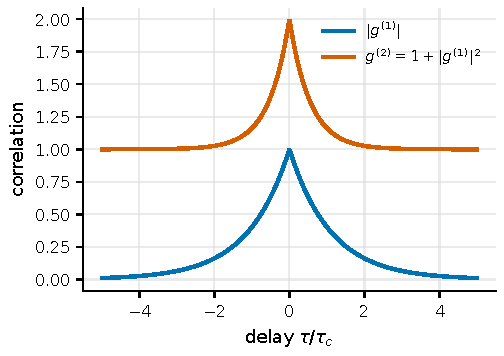
\includegraphics[width=0.86\linewidth]{figures/generated/chapter_04/ch04_siegert_relation.pdf}
\caption{Siegert 关系把一阶场相干的衰减，转化成二阶强度聚束峰。若 \(|g^{(1)}(\tau)|\) 随延迟以相干时间 \(\tau_c\) 衰减，则 \(g^{(2)}(\tau)-1\) 按 \(|g^{(1)}(\tau)|^2\) 衰减，并在大延迟回到无相关值 0；零延迟峰高在理想单模时为 1，真实观测还要乘上可见度因子 \(\zeta\)（模式数、偏振、背景；有限时间响应不含在 \(\zeta\) 内，另由卷积处理，见第 \ref{sec:e08-telescope} 节）。}
\label{fig:e08-siegert}
\end{figure}

\paragraph{谱形决定峰形；相干态是例外}
\label{sec:e08-shapes}

既然 \(g^{(1)}(\tau)\) 是谱线的傅里叶变换，那么\emph{谱线长什么样，聚束峰就长什么样}。三个常见谱形值得记住：

\begin{itemize}
  \item \textbf{矩形谱}（带宽 \(\Delta\nu\) 内平顶）：傅里叶变换是 sinc 函数，故 \(|g^{(1)}(\tau)|^2\propto{\rm sinc}^2(\Delta\nu\,\tau)\)——峰带旁瓣。
  \item \textbf{洛伦兹谱}（Lorentzian，如碰撞展宽或自然线宽）：\(|g^{(1)}(\tau)|=e^{-|\tau|/\tau_c}\) 是双边指数衰减，故 \(g^{(2)}-1\propto e^{-2|\tau|/\tau_c}\)——尖顶。
  \item \textbf{高斯谱}（Gaussian，如多普勒展宽）：傅里叶变换仍是高斯，故 \(|g^{(1)}(\tau)|^2\) 也是高斯——圆顶。
\end{itemize}

反过来用，就是一门实验技术：测出 \(g^{(2)}(\tau)\) 峰的\emph{宽度}，就能反推谱线宽度。对于像 \(\eta\) Carinae 附近那些天体激光候选谱线，普通光谱仪很难做到光谱分辨本领 \(R\equiv\lambda/\Delta\lambda\sim10^8\)（无量纲），而纳秒级的强度相关却能对 MHz 到 GHz 的线宽给出独立约束 \citep{2005NewA...10..361J,2008AIPC..984..216D,2014ApJ...789L..10T}。

但必须把\textbf{适用边界}钉死：Siegert 关系是\emph{高斯混沌光专属}的。理想相干态（激光）明明有很长的一阶相干（\(g^{(1)}\) 长程不衰减），可它的 \(g^{(2)}\equiv1\)——绝不满足 \(1+|g^{(1)}|^2\)。原因正是圆高斯假设不成立：相干态不是大量随机相位的叠加，它的场没有那种明暗斑纹起伏。同理，反聚束光、压缩光、单光子源、强非平稳脉冲，以及少数几个相干子源的叠加，都会打破式 \eqref{eq:e08-siegert}。天文上更常见的是混合场——许多非热小源平均后近似热光，或热连续谱上叠加一条窄非热线——用 Siegert 关系前，务必先确认光的"混沌"血统。

\section{从理想相关到望远镜里的估计量}
\label{sec:e08-telescope}

理想的 \(g^{(2)}\) 峰又窄又高（皮秒宽、峰高 1）。可探测器不是无限快的，它测到的是理想相关与\emph{仪器响应}的卷积：

\begin{equation}
  g_{\rm obs}^{(2)}(\tau)-1=\int_{-\infty}^{+\infty}
  \big[g_{\rm true}^{(2)}(\tau')-1\big]\,R_{\Delta t}(\tau-\tau')\,{\rm d}\tau',
  \label{eq:e08-response-conv}
\end{equation}
\begin{formulaexplain}
\(g_{\rm true}^{(2)}\) 是光场本征相关；\(g_{\rm obs}^{(2)}\) 是观测到的；\(R_{\Delta t}\) 是面积归一化为 1 的仪器响应函数（由探测器 jitter、电子带宽、采样窗口、分析 bin 共同决定）；\(\tau'\) 是积分变量。卷积会把窄峰拉宽、压低，但守住峰的面积。
\end{formulaexplain}

这里藏着一个容易误解的事实：卷积\emph{守面积、不守峰高}。一个面积固定的窄峰，被一个宽得多的响应抹开后，峰会变矮变胖。若内禀峰宽 \(\tau_c\) 远小于有效响应宽度 \(\Delta t_{\rm eff}\)，那么峰高近似按 \(\tau_c/\Delta t_{\rm eff}\) 这个比例被稀释。把这项时间稀释和上一节的模式、背景稀释合在一起，就得到望远镜里相关峰高的\emph{误差预算式}：

\begin{equation}
  C_{\rm obs}\equiv g_{\rm obs}^{(2)}(0)-1
  \simeq C_{\rm true}\,\frac{\tau_c}{\Delta t_{\rm eff}}\,\frac{1}{M}\,f_A f_B,
  \label{eq:e08-contrast}
\end{equation}
\begin{formulaexplain}
\(C_{\rm obs}\) 是观测峰高，\(C_{\rm true}\) 是理想峰高（单模热光为 1）；\(\tau_c/\Delta t_{\rm eff}\) 是时间稀释；\(M=M_{\rm pol}M_{\rm sp}\) 是偏振与空间模式数；\(f_A,f_B\) 是两通道里源光子占总计数的比例（背景稀释）。这是数量级公式，精确分析要把实测响应、谱形 \(|g^{(1)}|^2\)、背景一起放进模型。
\end{formulaexplain}

\begin{figure}[tbp]
\centering
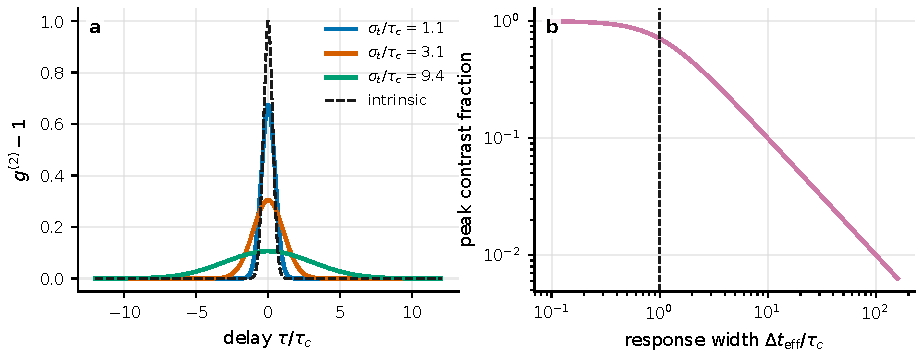
\includegraphics[width=0.95\linewidth]{figures/generated/chapter_04/ch04_response_convolution.pdf}
\caption{有限时间响应把窄的热光聚束峰拉宽、压低。左图虚线是内禀皮秒量级峰，实线是被不同响应宽度卷积后的观测峰；右图显示当 \(\Delta t_{\rm eff}\gg\tau_c\) 时，零延迟峰高近似按 \(\tau_c/\Delta t_{\rm eff}\) 下降——面积守住了，峰高被稀释。}
\label{fig:e08-response}
\end{figure}

\textbf{代进真实标尺：Guerin 恒星聚束实验。}\ Guerin 等人用 1 米望远镜、多模光纤、分束器、两只雪崩光电二极管（APD）和延迟直方图，测到了恒星的热光聚束 \citep{2017MNRAS.472.4126G}。他们的参数是一组极好的量级练习：中心波长约 \(7800\,\text{\AA}\)，最窄滤光片带宽 \(10\,\text{\AA}\)。先算相干时间（同式 \eqref{eq:e08-tauc}）：\(\Delta\nu\simeq c\Delta\lambda/\lambda^2\approx5\times10^{11}\,{\rm Hz}\)，故 \(\tau_c\simeq2\,{\rm ps}\)。而两个探测器的相对响应峰宽约 \(\Delta t_{\rm eff}\approx700\,{\rm ps}\)（单只 APD 的时间 jitter 约 500 ps）。理想热光 \(C_{\rm true}=1\)，仅时间稀释一项就给出 \(\tau_c/\Delta t_{\rm eff}\approx2/700\approx3\times10^{-3}\)。这已经是峰高的主导因子；在它之外，还要再乘上一个 \(\mathcal O(1)\) 的形状/模式系数——洛伦兹内禀峰与近高斯响应卷积后，零延迟峰高相对"面积除以响应宽"这一粗估会有一个约 \(0.7\) 的峰形折扣，加上残余的偏振/模式与背景稀释——把预期峰高压到

\[
  C_{\rm obs}\approx(2\text{--}3)\times10^{-3}\quad(\text{量级估计}),
\]

与实验室热源实测 \((2.01\pm0.09)\times10^{-3}\)、以及三颗亮星给出的约 \(1.8\)--\(2.0\times10^{-3}\) 的峰做数量级比较，符合得很好。结论一句话：望远镜相关图上直接冒出来的，绝不是教科书的 \(g^{(2)}(0)=2\)，而是 \(1+10^{-3}\)、\(1+10^{-6}\) 乃至更小的过量。看得见这个小数，靠的是海量事件对的累积。

\paragraph{延迟直方图：把事件表变成相关函数}
\label{sec:e08-histogram}

那么在事件表里，\(g^{(2)}\) 具体怎么估出来？答案是\textbf{延迟直方图}（delay histogram）。取两个通道 \(A,B\)，把每一对事件的时间差 \(t_{B,j}-t_{A,i}\) 都算出来，扔进宽为 \(\delta\tau\) 的延迟 bin 里累计：

\begin{equation}
  H_{AB}(\tau_m)=\sum_{i\in A}\sum_{j\in B}
  \mathbf{1}\!\left(\tau_m-\tfrac{\delta\tau}{2}\le t_{B,j}-t_{A,i}<\tau_m+\tfrac{\delta\tau}{2}\right),
  \label{eq:e08-histogram}
\end{equation}
\begin{formulaexplain}
\(H_{AB}(\tau_m)\) 是延迟落在第 \(m\) 个 bin（中心 \(\tau_m\)、宽 \(\delta\tau\)）里的事件对数；\(\mathbf 1(\cdot)\) 是示性函数，落进窗内取 1、否则取 0；双重求和遍历两通道所有事件对。它把事件表直接变成相关函数的原始计数。
\end{formulaexplain}

要把这个原始计数归一化成"无相关时等于 1"的 \(g^{(2)}\)，就除以随机符合的期望。设两通道平均计数率 \(r_A,r_B\)，总有效观测时长（live time）\(T\)：

\begin{equation}
  \widehat g^{(2)}_{AB}(\tau_m)=\frac{H_{AB}(\tau_m)}{r_A\,r_B\,\delta\tau\,T}.
  \label{eq:e08-estimator}
\end{equation}
\begin{formulaexplain}
\(\widehat g^{(2)}_{AB}\) 是二阶相关的估计量；分母 \(r_Ar_B\,\delta\tau\,T\) 是同样时长、同样 bin 宽、同样计数率下的随机符合期望。分子分母都是"对数"，比值无量纲，且在无相关时自动等于 1。
\end{formulaexplain}

分母的道理很直白：\(A\) 通道一共有 \(r_AT\) 个事件，对每个 \(A\) 事件，一个 \(B\) 事件恰好落进它 \(\delta\tau\) 窗口的概率是 \(r_B\delta\tau\)，两者相乘就是期望的随机符合数。实际分析常常不用这条解析分母，而是用大时间偏移、不同观测段、偏振错配或 off-source 通道构造一条参考直方图 \(H_{\rm ref}\)，再取比值——这样能吸收 TDC bin 宽不均、电子串扰、慢变透明度等系统效应。

\begin{figure}[tbp]
\centering
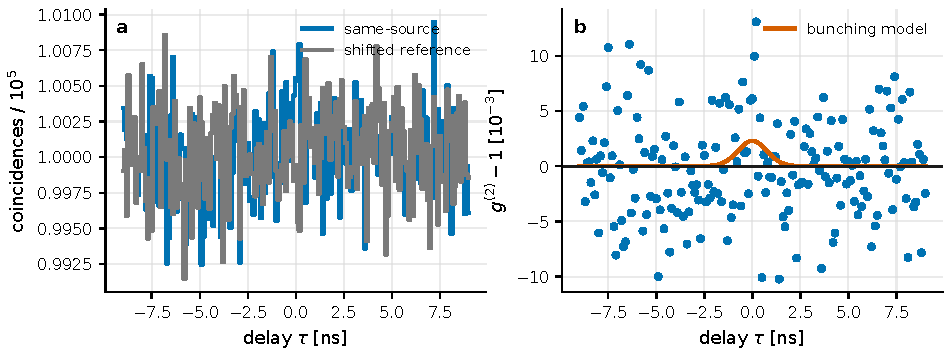
\includegraphics[width=0.95\linewidth]{figures/generated/chapter_04/ch04_delay_histogram_estimator.pdf}
\caption{延迟直方图估计量的结构。左图中同源事件对的直方图，在零延迟附近比移位的参考直方图多出很小的符合数；右图把差值按随机符合数归一化后得到 \(g^{(2)}-1\)，峰值只有 \(10^{-3}\) 量级。真实观测还要叠加死时间、背景和响应函数修正。}
\label{fig:e08-delay-hist}
\end{figure}

\paragraph{统计误差：一切都靠数够事件对}
\label{sec:e08-shotnoise}

估计量的精度从哪来？主要来自随机符合对数的散粒噪声。若某个延迟 bin 里随机符合数为 \(N_{\rm pair}\)，它是泊松涨落（第 \ref{chap:e03} 章），标准差 \(\sqrt{N_{\rm pair}}\)，相对误差就是

\begin{equation}
  \sigma\!\left[\widehat g^{(2)}(\tau)\right]\sim\frac{1}{\sqrt{N_{\rm pair}}}.
  \label{eq:e08-shotnoise}
\end{equation}
\begin{formulaexplain}
\(\sigma[\widehat g^{(2)}]\) 是相关估计量的统计误差；\(N_{\rm pair}=r_Ar_B\,\delta\tau\,T\) 是该 bin 的随机符合对数。要把误差压到 \(10^{-3}\) 以下的信号之下，就得积累巨量事件对。
\end{formulaexplain}

代进一组数字体会难度。取两个 \(r=10^{6}\,{\rm s^{-1}}\) 的通道、\(\delta\tau=100\,{\rm ps}=10^{-10}\,{\rm s}\)、\(T=1\,{\rm hr}=3600\,{\rm s}\)：
\[
  N_{\rm pair}=r_Ar_B\,\delta\tau\,T
  =(10^6)(10^6)(10^{-10})(3600)
  =3.6\times10^{5},
\]
故单 bin 统计误差 \(\sigma\sim1/\sqrt{3.6\times10^5}\approx1.7\times10^{-3}\)。这几乎和 Guerin 的信号 \(2\times10^{-3}\) 同量级——也就是说，一小时、单个延迟 bin 还远远不够，勉强只有 \(1\sigma\)。要把误差压到 \(10^{-4}\)，需要 \(N_{\rm pair}\sim10^{8}\)，也就是把事件对数从 \(3.6\times10^5\) 再积累约 \(300\) 倍（\(10^8/3.6\times10^5\approx278\)）。注意这 300 倍在两条路径上的标度并不相同：\(N_{\rm pair}\propto T\) 对曝光是线性的，故曝光时间需延长约 \(300\) 倍；而 \(N_{\rm pair}\propto r_Ar_B\) 对计数率是平方的，故两通道计数率各提高约 \(\sqrt{300}\approx17\) 倍即可（本章第 3 道"想一想"考的正是这个 \(r^2\) 标度）。当然也可以两者结合，或把聚束峰跨越的多个 bin 一起拟合（峰不止一个 bin 宽，可以联合利用）。这也提醒一个上限：当系统相关（TDC 串扰、背景归一化残差）停在 \(10^{-3}\) 量级时，继续加曝光并不能替代对这些系统项的修正。现代 VERITAS 与 MAGIC 强度干涉正是把这一思想，用离线相关、GPU/FPGA 相关器和多基线平均，推广到了空间尺度 \citep{2020NatAs...4.1164A,2024MNRAS.529.4387A}。

\section{前瞻：三阶相关与闭合相位}
\label{sec:e08-g3}

二阶相关只动用光子\emph{对}。如果同时保留三个望远镜（或三个通道），就能定义三阶强度相关：

\begin{equation}
  g^{(3)}_{123}=\frac{\big\langle I_1 I_2 I_3\big\rangle}
  {\big\langle I_1\big\rangle\big\langle I_2\big\rangle\big\langle I_3\big\rangle}.
  \label{eq:e08-g3}
\end{equation}
\begin{formulaexplain}
\(g^{(3)}_{123}\) 是三通道归一化强度相关；\(I_1,I_2,I_3\) 是三个望远镜的强度；分母是随机三重符合基线。它把统计对象从"光子对"推广到"光子三元组"。
\end{formulaexplain}

对高斯混沌光，同样用高斯矩定理把六阶矩拆开（这次是三个不带星号、三个带星号的场两两配对，"星号配非星号"的合法配对共 \(3!=6\) 个：其中 3 个把 \(I_i\) 就地配成 \(|\gamma|^2\) 型的模平方项，另外一对互为共轭的循环配对合成那个闭合项），结果里除了三条基线各自的模平方项，还多出一个\emph{三角形闭合}项：

\begin{equation}
  g^{(3)}_{123}=1+|\gamma_{12}|^2+|\gamma_{23}|^2+|\gamma_{31}|^2
  +2\,{\rm Re}\!\big(\gamma_{12}\,\gamma_{23}\,\gamma_{31}\big),
  \label{eq:e08-g3-closure}
\end{equation}
\begin{formulaexplain}
\(\gamma_{ij}\) 是通道 \(i,j\) 之间的一阶相干度（复数）；三个模平方项来自三条基线；末项 \({\rm Re}(\gamma_{12}\gamma_{23}\gamma_{31})\) 是三条基线相位相加后的\textbf{闭合相位}（closure phase）项。它是三阶强度干涉能触及相位组合的入口。
\end{formulaexplain}

关键在末项：\(\gamma_{12}\gamma_{23}\gamma_{31}\) 里三个复相干度的相位相加，恰好构成一个\emph{闭合三角}。二阶强度干涉只给 \(|\gamma|^2\)——把相位完全丢了；而三阶项里这个闭合相位是可测的。这正指向第 \ref{chap:e11} 章的成像相位问题：强度干涉天生丢相位，而闭合相位（以及高阶相关）是把相位组合找回来的一条路。代价是噪声大得多——光子三元组比光子对稀少得多，对系统误差也更敏感。Gamo 的早期理论、Nuñez 等人的成像模拟都把高阶相关视作强度干涉成像的重要延伸 \citep{1966JOSA...56..441G,2012MNRAS.419..172N}。

\begin{figure}[tbp]
\centering
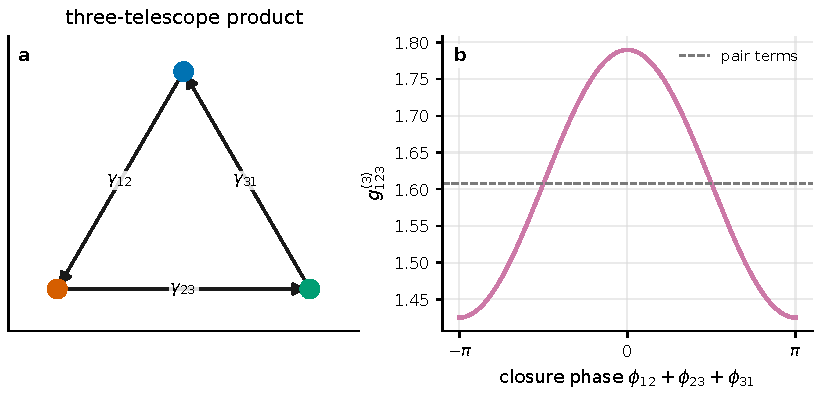
\includegraphics[width=0.92\linewidth]{figures/generated/chapter_04/ch04_g3_closure_phase.pdf}
\caption{三阶强度相关中闭合相位项的来源。左图中三台望远镜形成 \(\gamma_{12}\gamma_{23}\gamma_{31}\) 的闭合乘积；右图显示在固定 \(|\gamma_{ij}|\) 下，\(g^{(3)}\) 随闭合相位的余弦变化。二阶强度干涉只给 \(|\gamma|^2\)，三阶项才开始对相位组合敏感。}
\label{fig:e08-g3}
\end{figure}

\section{一扇门：把时间延迟换成空间基线}
\label{sec:e08-gateway}

本章从头到尾都在讲"时间延迟 \(\tau\)"——同一束光隔了 \(\tau\) 的呼应。最后一步，是把这套语言里的 \(\tau\) 换成\emph{空间基线} \(\bm B\)，一扇通往第 \ref{chap:e10} 章的门就打开了。

想象两台相隔 \(\bm B\) 的望远镜同时盯着同一颗恒星，各自记录强度涨落。把 \(g^{(1)}\) 的两个"时刻"换成两个"位置"，它就不再量"电场隔 \(\tau\) 记得多少相位"，而是量"相距 \(\bm B\) 的两点上电场有多相干"。而 van Cittert--Zernike 定理（第 \ref{chap:e10} 章会证）会告诉我们：这个空间版的 \(g^{(1)}(\bm B)\)，正是天空亮度分布的\textbf{复可见度}（complex visibility）——它是天体角结构的傅里叶分量。于是 Siegert 关系原样搬过来：

\[
  g^{(2)}(\bm B)-1=\zeta\,\big|g^{(1)}(\bm B)\big|^2
  =\zeta\,\big|V(\bm B)\big|^2 ,
\]

两台望远镜强度涨落的\emph{同步程度}，就直接给出复可见度的模平方 \(|V(\bm B)|^2\)。这就是 HBT 强度干涉的全部魔法：不必像振幅干涉那样把两台望远镜的电场用真空管道合束（那对光路稳定度的要求近乎苛刻），只靠事后比对两地各自记录的强度起伏，就能测到可见度模平方，进而反推恒星角直径。成立的前提，仍是本章反复强调的两条：源光近似高斯混沌光，且仪器归一化没把背景、模式数、时间响应混进 \(\zeta\)。

带着这扇门，我们就能走进第 \ref{chap:e10} 章——把"时间相关"升级成"空间相关"，把"相干时间"升级成"可见度曲线"，最终在第 \ref{chap:e11} 章从可见度反推出天体的像。

\section{本章要点}
\label{sec:e08-summary}

\begin{itemize}
  \item \textbf{两阶相干，两个朴素问题。}一阶 \(g^{(1)}(\tau)\)（式 \eqref{eq:e08-g1}）量电场的相位记忆：\(|g^{(1)}|\to1\) 相干、\(\to0\) 失忆，其衰减宽度就是相干时间 \(\tau_c\simeq1/\Delta\nu\)（780\,nm/1\,nm 给 \(\tau_c\approx2\,{\rm ps}\)）。二阶 \(g^{(2)}(\tau)\)（式 \eqref{eq:e08-g2-field}）量光子成对倾向。
  \item \textbf{三种统计三种峰。}泊松（相干态）\(g^{(2)}=1\)；热光聚束 \(g^{(2)}(0)=2\)；\(g^{(2)}(0)<1\) 反聚束，是非经典判据。经典写法 \(g^{(2)}=\langle II\rangle/\langle I\rangle^2\) 好用，但要警惕 \(I\) 是否已被响应卷积。
  \item \textbf{Siegert 关系是本章的桥。}\(g^{(2)}(\tau)=1+\zeta|g^{(1)}(\tau)|^2\)（式 \eqref{eq:e08-siegert}），来自高斯混沌光的四阶矩拆分（高斯矩/Wick 定理）：\(\langle II\rangle=\langle I\rangle^2+|G^{(1)}|^2\)。它让强度相关直接读出场相干模平方。谱形定峰形：矩形 sinc\(^2\)、洛伦兹指数、高斯高斯。\(\zeta\) 只收集模式、偏振、背景（有限时间响应另由卷积处理，不含在 \(\zeta\) 内）。\emph{对相干态不成立}。
  \item \textbf{望远镜里的稀释。}有限响应卷积守面积不守峰高，\(C_{\rm obs}\simeq C_{\rm true}(\tau_c/\Delta t_{\rm eff})(1/M)f_Af_B\)（式 \eqref{eq:e08-contrast}）。Guerin 实验：\(7800\,\text{\AA}\)、\(10\,\text{\AA}\)、\(\tau_c\approx2\,{\rm ps}\)、响应 \(\approx700\,{\rm ps}\)，观测峰只有 \(C_{\rm obs}\approx2\times10^{-3}\)。
  \item \textbf{估计量与噪声。}延迟直方图 \(\widehat g^{(2)}=H_{AB}/(r_Ar_B\,\delta\tau\,T)\)（式 \eqref{eq:e08-estimator}），误差 \(\sigma\sim N_{\rm pair}^{-1/2}\)（式 \eqref{eq:e08-shotnoise}）——一切靠数够事件对。
  \item \textbf{两扇门。}三阶 \(g^{(3)}\) 的闭合相位项通向第 \ref{chap:e11} 章的成像相位；把 \(\tau\) 换成基线 \(\bm B\)，\(g^{(1)}\) 就成了复可见度 \(V(\bm B)\)，通向第 \ref{chap:e10} 章的空间强度干涉。
\end{itemize}

\medskip
\noindent\textbf{想一想。}
\begin{enumerate}
  \item 把滤光片带宽从 \(10\,\text{\AA}\) 放宽到 \(100\,\text{\AA}\)，相干时间 \(\tau_c\) 怎么变？在响应 \(\Delta t_{\rm eff}\approx700\,{\rm ps}\) 不变的情况下，观测峰高 \(C_{\rm obs}\) 会升还是降，约变几倍？
  \item 有人测到某光源 \(g^{(1)}\) 在很长延迟内仍接近 1，却发现 \(g^{(2)}\equiv1\)。这更可能是热光还是激光？为什么它不违反 Siegert 关系？
  \item 若把两个通道的计数率各提高 10 倍、曝光时间加长 4 倍，单 bin 的随机符合数 \(N_{\rm pair}\) 变几倍？相应的统计误差 \(\sigma[\widehat g^{(2)}]\) 又变几倍？
\end{enumerate}
